\section{Requirements}

  This chapter lists the requirements of the system by extracting the use cases from the goal of the research project and its priorities. 

  \subsection{Use Cases}
    \label{use_cases}

    A use case diagram is created to better visualize the flow and possible use cases of the system on a high level based on the goal of the research project.

    \begin{figure}[!ht]
     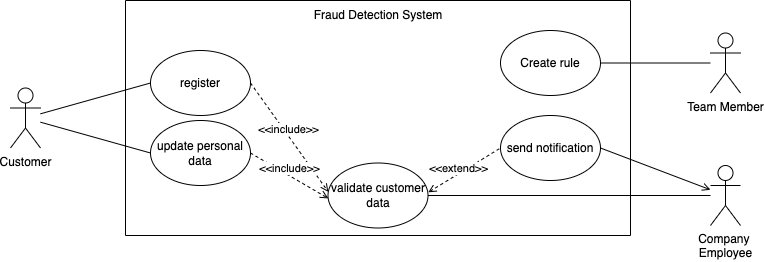
\includegraphics[width=\textwidth]{diagrams/use-case-diagram.png}
     \caption{Use case diagram of the fraud detection system}
     \label{fig:use_cases}
    \end{figure}

    The use case diagram gives a visual representation of the main functionality of the system as well as the actor involved in the process. The customer data validation will be run whenever a customer registers or updates his/her personal data. By running a validation whenever an operation on personal data is executed, the system would ideally validate and identify fraudulent customer as soon as possible. 
    
    Whenever a fraudulent customer is identified, a notification will be sent to concerned parties, so that necessary actions (for example, blocking the customer) can be taken as soon as possible. 

    The diagram also visualizes a use case of a validation rule creation by a team member, as a form of contribution based on his/her knowledge of a fraudulent customer with the intention to improve the reliability of the validation process.
    
  \newpage
  \subsection{User Stories}
    \label{user_stories}

    Based on the use cases visualized on \autoref{fig:use_cases}, the following user stories can be defined:

    \begin{itemize}
      \item \textbf{Verifying Customer Early}
        \begin{itemize}[label={},leftmargin=*]
          \item As a stakeholder, I want to verify customers, so that the company can have more confidence that the existing user base is trustworthy 
        \end{itemize}

      \item \textbf{Notification on Suspicious Cases}
        \begin{itemize}[label={},leftmargin=*]
          \item As an employee, I want to be notified when a user seems suspicious, so that I can do necessary actions accordingly
        \end{itemize}

      \item \textbf{Validation Rules Management}
        \begin{itemize}[label={},leftmargin=*]
          \item As an employee, I want to manage my own rule to validate users, so that I can use my expertise to find suspicious customers as efficiently as possible without the communication overhead with other teams
        \end{itemize}
    \end{itemize}

    The user stories listed above are the main requirements of the system. The functionalities of the system will be defined and implemented based on these user stories.
    
  \subsection{Software Quality Standard}
    \label{criteria}

    The system and software quality models defined in ISO 25010 \autocite{iso-2011} are used to establish a base on how to evaluate the quality of the system made for this research project. The table below contains a list of criteria taken from the software quality characteristics and its sub-characteristics described in ISO 20510, the meaning of each sub-characteristic and its importance to the research project. The criteria will be revisited during evaluation to assess the quality of the software made during the research project. 

     \begin{tabularx}{\linewidth}{p{0.3\textwidth} p{0.5\textwidth} p{0.2\textwidth}}
       \caption{Systems and software quality standard based on ISO 25010 and its importance} \\
        \toprule
        & Overview & Importance \\
        \midrule

        \multicolumn{3}{@{}l}{\textbf{Functional stability}}\\
        Completeness & System covers all the specified tasks listed on the requirement analysis & Very important \\
        Correctness & System provides correct results of the tasks listed on the requirement analysis & Very important \\
        Appropriateness & System accomplishes to fulfill the tasks listed on the requirement analysis in a well manner & Important \\

        \multicolumn{3}{@{}l}{\textbf{Reliability}}\\
        Maturity & System is stable during every day use & Important \\
        Availability & System is operational and accessible (ideally via a web browser and no installation is needed) & Very important \\
        Fault tolerance & System still operates well enough, despite software fault & Important \\
        Recoverability & System can recover data in the event of an interruption or failure & Very important \\

        \multicolumn{3}{@{}l}{\textbf{Performance efficiency}}\\
        Time behavior & Response and processing time of the system is reasonable & Important \\
        Resource Utilization & The amount and types of resources used by the system is kept as minimum as possible & Not important \\
        Capacity & Maximum limits of a system parameter is within a reasonable range for everyday use & Not important \\

        \multicolumn{3}{@{}l}{\textbf{Usability}}\\
        Appropriateness Recognizability & It can be easily recognized, that the system is suitable for the current user need & Not important \\
        Learnability & It's easy to learn how to use the system & Not important \\
        Operability & The system is easy to operate & Very important \\
        User Error Protection & System can protect or prevent users against making errors &Somewhat important \\
        User Interface Aesthetics & User interface is aesthetically pleasing & Very important \\
        Accessibility & System can be used with the widest range of characteristics and capabilities & Not important \\

        \multicolumn{3}{@{}l}{\textbf{Security}}\\
        Confidentiality & System is able to ensure that data is only accessible to those who have authorized access &Somewhat important \\
        Integrity & System is able to prevent unauthorized access and modification to computer programs &Somewhat important \\
        Non-repudiation & Actions or events can be proven to have taken place & Somewhat important \\
        Accountability & Actions of an unauthorized user can be traced back & Not important \\
        Authenticity & How well the identity of a subject / resource can be proved & Not important \\

        \multicolumn{3}{@{}l}{\textbf{Compatibility}}\\
        Co-existence & Each component of the system can work efficiently without any bottleneck while sharing the same environment & Somewhat important \\
        Interoperability & Two or more systems, products, or components are able to exchange information and use it & Very important \\

        \multicolumn{3}{@{}l}{\textbf{Maintainability}}\\
        Modularity & Component of system can be changed with minimal impact on the other component & Important \\
        Reusability & Assets can be used in more than one component & Not important \\ 
        Analysability & Activities within the system can be easily analyzed (e.g.: in form of logging) & Somewhat important \\
        Modifiability & System can be modified without introducing defects or degrading existing product quality & Very important \\
        Testability & Test criteria for a system is effective and preferably can be run automatically & Very important \\

        \multicolumn{3}{@{}l}{\textbf{Portability}}\\
        Adaptability & System can be adapted for different or evolving HW, SW or other usage environment & Not important \\
        Installability & System can be un- and/or installed successfully & Important \\
        Replaceability & System as a product can replace another comparable product & Not important \\

        \bottomrule
      \end{tabularx}

      \newpage

    